\documentclass[a4paper]{article}
\usepackage[francais]{babel}
\usepackage{fontspec}
\usepackage{enumitem}
\usepackage{authblk}
\usepackage{minted}
\usepackage{amsmath}
\usepackage{tabularx}
\newcolumntype{C}[1]{>{\centering\arraybackslash}p{#1}}
\setlength{\parindent}{0pt}
\usepackage{hyperref}
\hypersetup{
    colorlinks,
    citecolor=black,
    filecolor=black,
    linkcolor=black,
    urlcolor=blue
}
\usepackage{etoolbox}
\patchcmd{\thebibliography}{\section*{\refname}}{}{}{}
\usepackage[left=2.5cm,top=2.5cm,right=2.5cm,bottom=2.5cm]{geometry}

\title{MyLab2 GB \protect\\ Emulateur de Gameboy sur MyLab2}
\author{Orphée Antoniadis}
\affil{\small Projet de semestre - Prof. Fabien Vannel}
\affil{\small Hepia ITI 3\up{ème} année}
\date{Semestre d'automne 2017-2018}

\begin{document}
\maketitle

\vspace*{\stretch{1}}
\begin{figure}[!h]
  \centering
  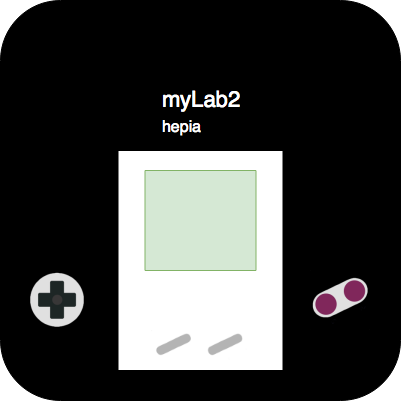
\includegraphics[scale=0.7]{images/mylab2gb.png}
\end{figure}
\vspace*{\stretch{1}}

\begin{figure}[!b]
	\centering
	\begin{minipage}{.5\textwidth}
		\centering
		
\includegraphics[width=.6\linewidth]{images/hepia.jpg}
	\end{minipage}%
	\begin{minipage}{.5\textwidth}
		\centering
		
\includegraphics[width=.6\linewidth]{images/hesso.jpg}
	\end{minipage}
\end{figure}
\newpage

\newpage
\setcounter{tocdepth}{3}
\tableofcontents
\newpage

%%%%%%%%%%%%%%%%%%%%%%%%%%%%%%%%%%%%%%%%%%%%%%%%%%%%%%%%%%%%%%%%%%
%%%%%%%%%%%%%%%%%%%%%%%%%%%%%%%%%%%%%%%%%%%%%%%%%%%%%%%%%%%%%%%%%%

\section{Introduction}
\subsection{Objectif}
L'objectif principal de ce projet était de développer un émulateur de la console
de jeux vidéos de Nintendo appelée Gameboy pour la carte de d'extension MyLab2
développée à hepia. Un emulateur est un logiciel permettant d'imiter le comportement
physique d'un matériel informatique. Le but ici est donc d'imiter le comportement
du processeur de la Gameboy avec tous ces périphériques. Nous allons voir dans
un premier temps les caractéristiques de la MyLab2 ainsi que de ces périphériques.
Nous allons ensuite regarder comment fonctionne la Gameboy. L'émulateur sera
finalement présenté avec tout son fonctionnement mais aussi les problèmes rencontrés
et la manière dont ils ont été résolus.

%%%%%%%%%%%%%%%%%%%%%%%%%%%%%%%%%%%%%%%%%%%%%%%%%%%%%%%%%%%%%%%%%%

\subsection{Méthode}
Il a fallut dans un premier temps comprendre le fonctionnement de la Gameboy. 
Le projet a donc commencé par un travail de recherche et de documentation. Etant 
donné que Nintendo n'a jamais rendu public la datasheet de sa console, toutes les 
informations récoltées ont été obtenues après un travail de reverse engineering 
effectuée par la communauté. Heureusement, la communauté de développeurs d'émulateurs 
est très active, de nombreux forums et blogs existent ce qui a simplifié la recherche
d'informations. Toutes les sources que j'ai trouvé seront listées à la fin de se 
document et pourront faire office de base de donnée complète pour quiconque voulant 
en apprendre plus sur la console ou bien même voulant développer son propre émulateur.
Ce n'est qu'ensuit que le travail de développement de l'émulateur a commencé. Ce
projet de semestre a donc suivi les étapes suivantes.
\begin{itemize}[label=\textbullet]
	\item Travail de recherche
	\item Implémentation de l'émulateur
	\item Tests avec la MyLab2
\end{itemize}

%%%%%%%%%%%%%%%%%%%%%%%%%%%%%%%%%%%%%%%%%%%%%%%%%%%%%%%%%%%%%%%%%%

\subsection{Schéma}
\begin{figure}[!h]
  \centering
  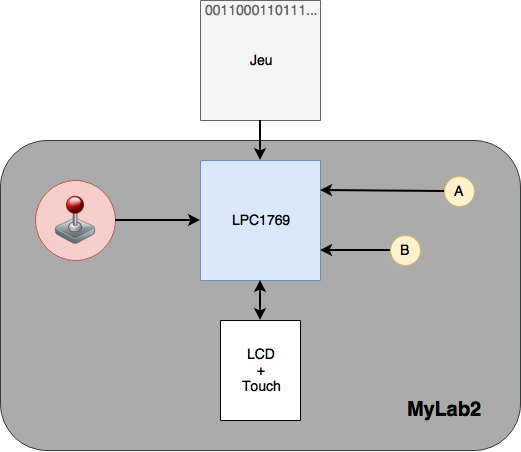
\includegraphics[scale=0.6]{images/schema_systeme.png}
  \caption{Schéma explicatif du projet}
\end{figure}

\newpage
%%%%%%%%%%%%%%%%%%%%%%%%%%%%%%%%%%%%%%%%%%%%%%%%%%%%%%%%%%%%%%%%%%
%%%%%%%%%%%%%%%%%%%%%%%%%%%%%%%%%%%%%%%%%%%%%%%%%%%%%%%%%%%%%%%%%%

\section{MyLab2}

\begin{figure}[!h]
  \centering
  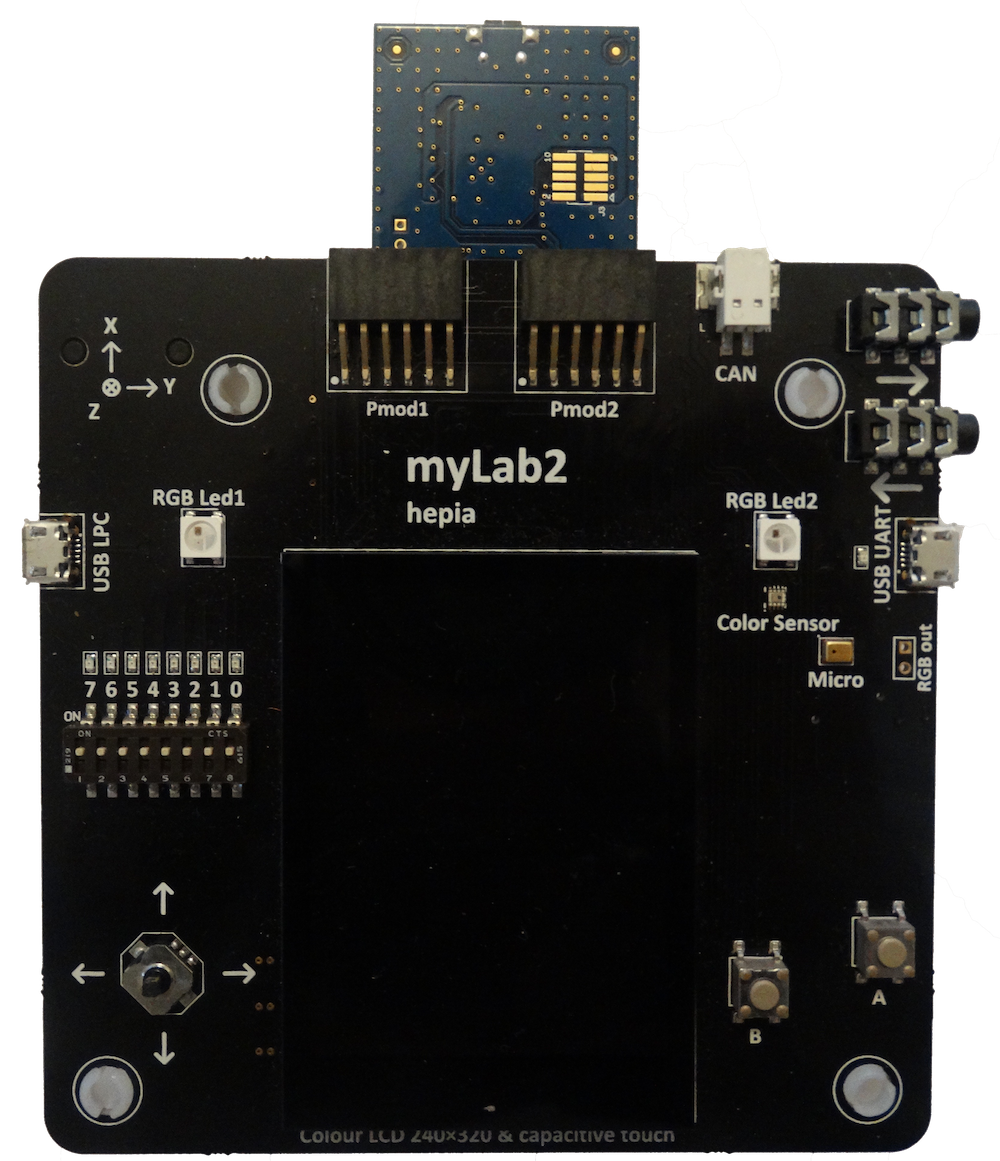
\includegraphics[scale=0.3]{images/mylab2.png}
  \caption{La MyLab2}
\end{figure}

\subsection{Introduction}
La MyLab2 est une carte d'extension pour les kits de développement des microcontrolleurs
LPC1769 et LPC4337 de NXP. Cette carte a été développée à hepia, au laboratoire
de systèmes numériques. Elle vient se superposer aux cartes de NXP via des connecteurs
broches. \\

Le LPC1769 de NXP est un microcontrolleur ARM Cortex-M3 ayant une fréquence d'horloge
pouvant aller jusqu'à 120MHz. Ce dernier propose une mémoire flash de 512kB (mais
seulement la moitié est programmable avec la version gratuite de LPCXpresso) ainsi
qu'une SRAM de 64kB. A noter que les 64kB de SRAM sont discontinus et qu'il y a en
réalité deux banques de RAM de 32kB chacune. 
Le LPC4337 de NXP est un microcontrolleur ARM Cortex-M4 ayant une fréquence d'horloge 
pouvant aller jusqu'à 204MHz mais inclut aussi un coprocesseur ARM Cortex-M0 pouvant
aller à la même fréquence d'horloge. La SRAM de ce dernier fait 136kB. \\

Pour ce projet, le microcontrolleur utilisé sera le LPC1769 pour un soucis pratique.
En effet, nous avons déjà eu à utiliser cette carte pour le cours de microcontrolleurs
et périphériques de deuxième année ce qui fait que j'avais déjà une grande partie de
la librairie de gestion des périphériques de la carte d'extension prête. C'était un
gain de temps non négligeable qui m'a permis de me concentrer sur l'émulation de
la Gameboy. \\

Le projet pourrait tout de même être repris et porté sur le LPC4337 afin d'avoir de
meilleures performances étant donné que sa fréquence d'horloge est deux fois plus
grande, qu'il dispose de deux processeurs permettant une parallélisation des taches
et qu'il y a plus de RAM.

\newpage

%%%%%%%%%%%%%%%%%%%%%%%%%%%%%%%%%%%%%%%%%%%%%%%%%%%%%%%%%%%%%%%%%%

\subsection{Périphériques utilisés}
\subsubsection{Boutons}
Les boutons A et B de la MyLab2 sont de simples pins GPIO. Le LPC1769 propose
des interruptions ($\overline{EINT3}$) sur les ports 0 et 2 du GPIO. Ici, le bouton A est sur la pin
10 du port 2 (P2.10) et le bouton B est sur la pin 19 du port 0 (P0.19). L'interruption
peut se faire sur le flanc montant ou descendant (ou les deux). Pour l'activer,
il faut mettre le bit correspondant à 1 dans le registre \mintinline{c}{IntEnF}
(flanc descendant) ou \mintinline{c}{IntEnR} (flanc montant). Lors d'une interruption,
il faut regarder laquelle a eu lieu dans le registre \mintinline{c}{IntStatF}/\mintinline{c}{IntStatR}
puis la quittancer en mettant le bon bit à 1 dans le registre \mintinline{c}{IntClr}.

\subsubsection{Joystick}
Le joystick de la MyLab2 est aussi relié à une pin GPIO mais contrairement aux
boutons A et B, il est relié au port 1 du GPIO. Il n'y a pas d'interruptions
sur le port 1 du GPIO, il faut donc vérifier l'état des pins du joystick de manière
régulière. Pour se faire, un timer sera utilisé qui provoquera une interruption
($\overline{TIMER0}$) toutes les 10ms. La routine d'interruption appelle la fonction \mintinline{c}{joystick_handler}
qui prend comme argument une fonction de callback (un pointeur sur une fonction
qui sera appelée si une des directions du joystick est appuyée), l'argument de cette 
dernière, et le mode de vérification (\mintinline{c}{POLLING} ou \mintinline{c}{TRIGGER}). 
En mode \mintinline{c}{POLLING}, la fonction de callback sera appelée qu'une seule
fois si le joystick est maintenu appuyé contrairement au mode \mintinline{c}{TRIGGER}
où la fonction sera appelée tant que le joystick n'est pas relâché. La fonction de
callback doit avoir comme prototype:

\inputminted[breaklines,breaksymbol=,linenos,frame=single,stepnumber=5,tabsize=2,firstline=14,lastline=14]
{c}{../../workspace/mylab2-gb/src/controls.c}

avec \mintinline{c}{pos} qui est la position du joystick, \mintinline{c}{edge} qui
est le flanc (montant ou descendant) et \mintinline{c}{arg} qui contient l'argument
de la fonction (peut être à \mintinline{c}{NULL}).

\subsubsection{Ecran LCD}
La MyLab2 utilise le le bus de communication SPI pour communiquer avec l’écran. 
Afin d'initialiser le SPI, il faut d'abord sélectionner les bonnes pins dans les 
registres appropriés (\mintinline{c}{PINSEL0} et \mintinline{c}{PINSEL1}). En effet, 
les pins sont configurées par défaut sur des pins GPIO. Pour le LPC1769 ce sont 
donc les bits 31:30 de \mintinline{c}{PINSEL0} et 5:0 de \mintinline{c}{PINSEL1} 
qu'il faut modifier. \\

Il faut ensuite fixer la valeur de la fréquence de transmission. Un registre de configuration du
SPI le permet. C'est le registre \mintinline{c}{SPCCR}. La valeur
donné à ce registre va diviser la valeur de l'horloge du SPI. Pour atteindre
une fréquence de transmission maximale, il faut mettre l'horloge du SPI à 100MHz
en modifiant le registre \mintinline{c}{PCLKSEL0} puis fixer la valeur du registre
\mintinline{c}{SPCCR} à 10 pour avoir une fréquence de transmission de 10MHz ($\frac{100}{10}$).
Pour finir il faut juste activer la communication SPI en la mettant en master mode.
Ceci se fait dans le registre \mintinline{c}{SPCR} (bit 5 à 1). \\

L'écriture et la lecture du bus SPI se fait à l'aide du même registre pour le
LPC1769. Ce registre est le registre  \mintinline{c}{SPDR}. Pour écrire,
il faut fixer la valeur du registre aux données à envoyer puis attendre que le flag
de confirmation d'envoi soit mis à 1. Ce flag est le bit 7 du registre \mintinline{c}{SPSR}.
\newline
Pour venir lire sur le bus SPI, il faut d'abord envoyer 0xFF (donc en utilisant
la fonction d'écriture) puis venir lire sur ce même registre (buffer bi-directionnel). \\

L'écran LCD accepte 2 types de données, les instructions et les arguments
d'instruction. La pin DC (pin GPIO 1.16) permet de contrôler ce qui va être envoyé.
Le DC est à 0 lors de l'envoi d'une instruction et à 1 pour l'envoi d'un argument.
La liste complète des instructions est disponible dans la documentation de l'écran
LCD. Pour ce projet, seulement 3 de ces instructions sont utilisées. Celle pour séléctionner
la colonne d'écriture en pixels (instruction 0x2A), celle pour séléctionner la ligne
d'écriture en pixels (instruction 0x2B) et enfin, celle pour écrire dans la mémoire
de l'écran (instruction 0x2C). La mémoire est l'ensemble des données qui composent
l'intégralité des pixels de l'écran. Ici l'écran est de $240 \times 320$ et un pixel
est codé sur 16 bits donc la mémoire serait ces $240 \times 320 \times 16$ bits.
Pour allumer un pixel sur l'écran, il faut d'abord séléctionner la zone d'écriture
en utilisant les instructions 0x2A et 0x2B, puis il faut écrire les données relatives 
à la couleur du pixel désirée en utilisant l'instruction 0x2C).

\subsubsection{Dalle tactile}
La MyLab2 communique avec la dalle tactile en utilisant le bus I$^2$C. La détection 
d'appuie sur la dalle tactile se fait quand à elle par interruption GPIO. Il faut
donc activer d'abord ces interruptions (comme pour les boutons A et B) puis récupérer 
les informations voulues dans la routine d'interruption. Les informations sont par 
exemple les coordonnées de position et peuvent être lues dans les registres de la 
dalle tactile dont les adresses sont disponibles dans la documentation. Pour ce projet, 
il n'y a eu besoin que de récupérer des coordonnées de la position détectée. Pour
récupérer  ces informations, il faut d'abord envoyer (donc écrire sur le bus I$^2$C)
l'adresse du registre à lire et ensuite venir lire dans ce registre. \\

A noter qu'il faut bien entendu initialiser le bus I$^2$C ce qui est fait relativement de la même
manière que le bus SPI. Petite différence juste pour fixer la fréquence de transmission
qui se fait par deux registres, les registres \mintinline{c}{I2SCLH} et \mintinline{c}{I2SCLL}.
Ces registres correspondent respectivement à la fréquence de l'horloge à l'état haut et à l'état
bas. La fréquence du bus I$^2$C en fast mode est de 400kHz et l'horloge périphérique
est à 25MHz par défaut donc il faut mettre ces deux registres à 32 ($\frac{25000}{32+32}=400$).
Il faut pour finir activer les interruptions I$^2$C et créer l'algorithme représenté
par un organigramme dans la documentation du LPC1769.

\subsubsection{UART}
Le périphérique UART de la MyLab2 peut être utilisé pour communiquer des informations
depuis la carte vers une machine hôte. L'UART peut par exemple être utilisé pour
envoyer des logs du microcontrolleur. Comme pour les bus SPI et I$^2$C, l'UART
doit d'abord être initialiser en séléctionnant les bonnes pins dans les registres
\mintinline{c}{PCONP}, \mintinline{c}{PINSEL0}. Il faut ensuite mettre le registre
\mintinline{c}{LCR} de l'UART à la valeur 0x80 afin d'indiquer d'autoriser l'accès aux diviseurs 
d'horloge. Ces diviseurs sont les registres \mintinline{c}{FDR}, \mintinline{c}{DLM}
et \mintinline{c}{DLM} et ils fixent la valeur de baudrate de la transmission.
Le calcul pour trouver leurs valeurs est le suivant:
\begin{equation*}
	UART_{baudrate}=\frac{PCLK}{16 \times (256 \times DLM \times DLL) \times (1 + \frac{DivAddVal}{MulVal})}
\end{equation*}
$DivAddVal$ contient les 4 bits de poids faible du registre \mintinline{c}{FDR} et
$MulVal$ ces 4 bits de poids fort. De plus leurs valeurs doivent respecter les conditions
suivantes:
\begin{itemize}[label=\textbullet]
	\item $1 \leq MulVal \leq 15$
	\item $0 \leq DivAddVal \leq 14$
	\item $DivAddVal < MulVal$ 
\end{itemize}
Après avoir fixé le baudrate, il faut désactiver l'accès aux diviseurs d'horloge
et fixer la transmission à 8 bits (5 bits par défaut) en mettant le regsitre
\mintinline{c}{LCR} à 0x03. Pour finir, la communication UART peut être activée
en mettant le registre \mintinline{c}{FCR} à 1. La communication se fera en utilisant
le registre \mintinline{c}{THR}.

\newpage

%%%%%%%%%%%%%%%%%%%%%%%%%%%%%%%%%%%%%%%%%%%%%%%%%%%%%%%%%%%%%%%%%%
%%%%%%%%%%%%%%%%%%%%%%%%%%%%%%%%%%%%%%%%%%%%%%%%%%%%%%%%%%%%%%%%%%

\section{Gameboy}

\begin{figure}[!h]
  \centering
  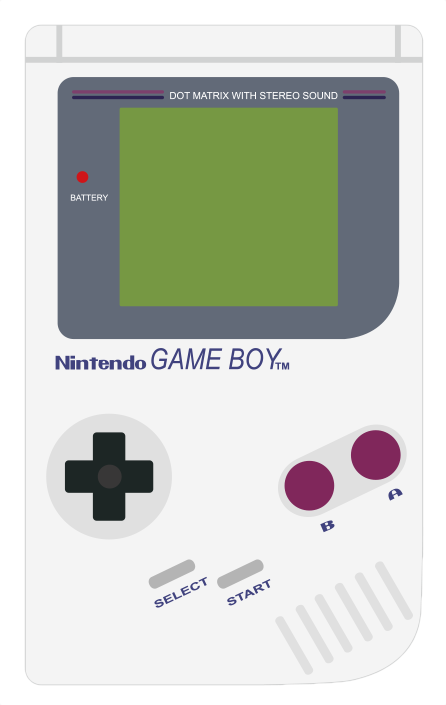
\includegraphics[scale=0.5]{images/gameboy.png}
  \caption{La Gameboy}
\end{figure}

\subsection{Introduction}
La Gameboy est une console de jeux vidéos portable 8 bits développée et fabriquée
par la firme japonaise Nintendo. La console a été mise en vente en 1989 et a connu
un franc succès à travers le monde jusqu'à la fin de sa production en 2003.
Nous allons dans cette partie étudier les caractéristiques et les périphériques
de la console. \\

Le processeur de la Gameboy est le LR35902, processeur semblable au Zilog Z80 et
cadensé à 4,19MHz. La mémoire de la console est de 64kB. Elle possède quatre boutons, 
A, B, START et SELECT, une croix directionnelle et une fente pour insérer les 
cartouches de jeux qui était située sur le haut, à l'arrière de la console. Elle est
aussi dotée de hauts parleurs et d'un port série pour la communication entre deux
consoles. Le son et la communication série ne seront pas emulés pour ce projet
mais une amélioration future pourrait les rajouter. Divisons donc toutes ces parties
en blocs.

\newpage

%%%%%%%%%%%%%%%%%%%%%%%%%%%%%%%%%%%%%%%%%%%%%%%%%%%%%%%%%%%%%%%%%%

\subsection{CPU}

\begin{figure}[!h]
  \centering
  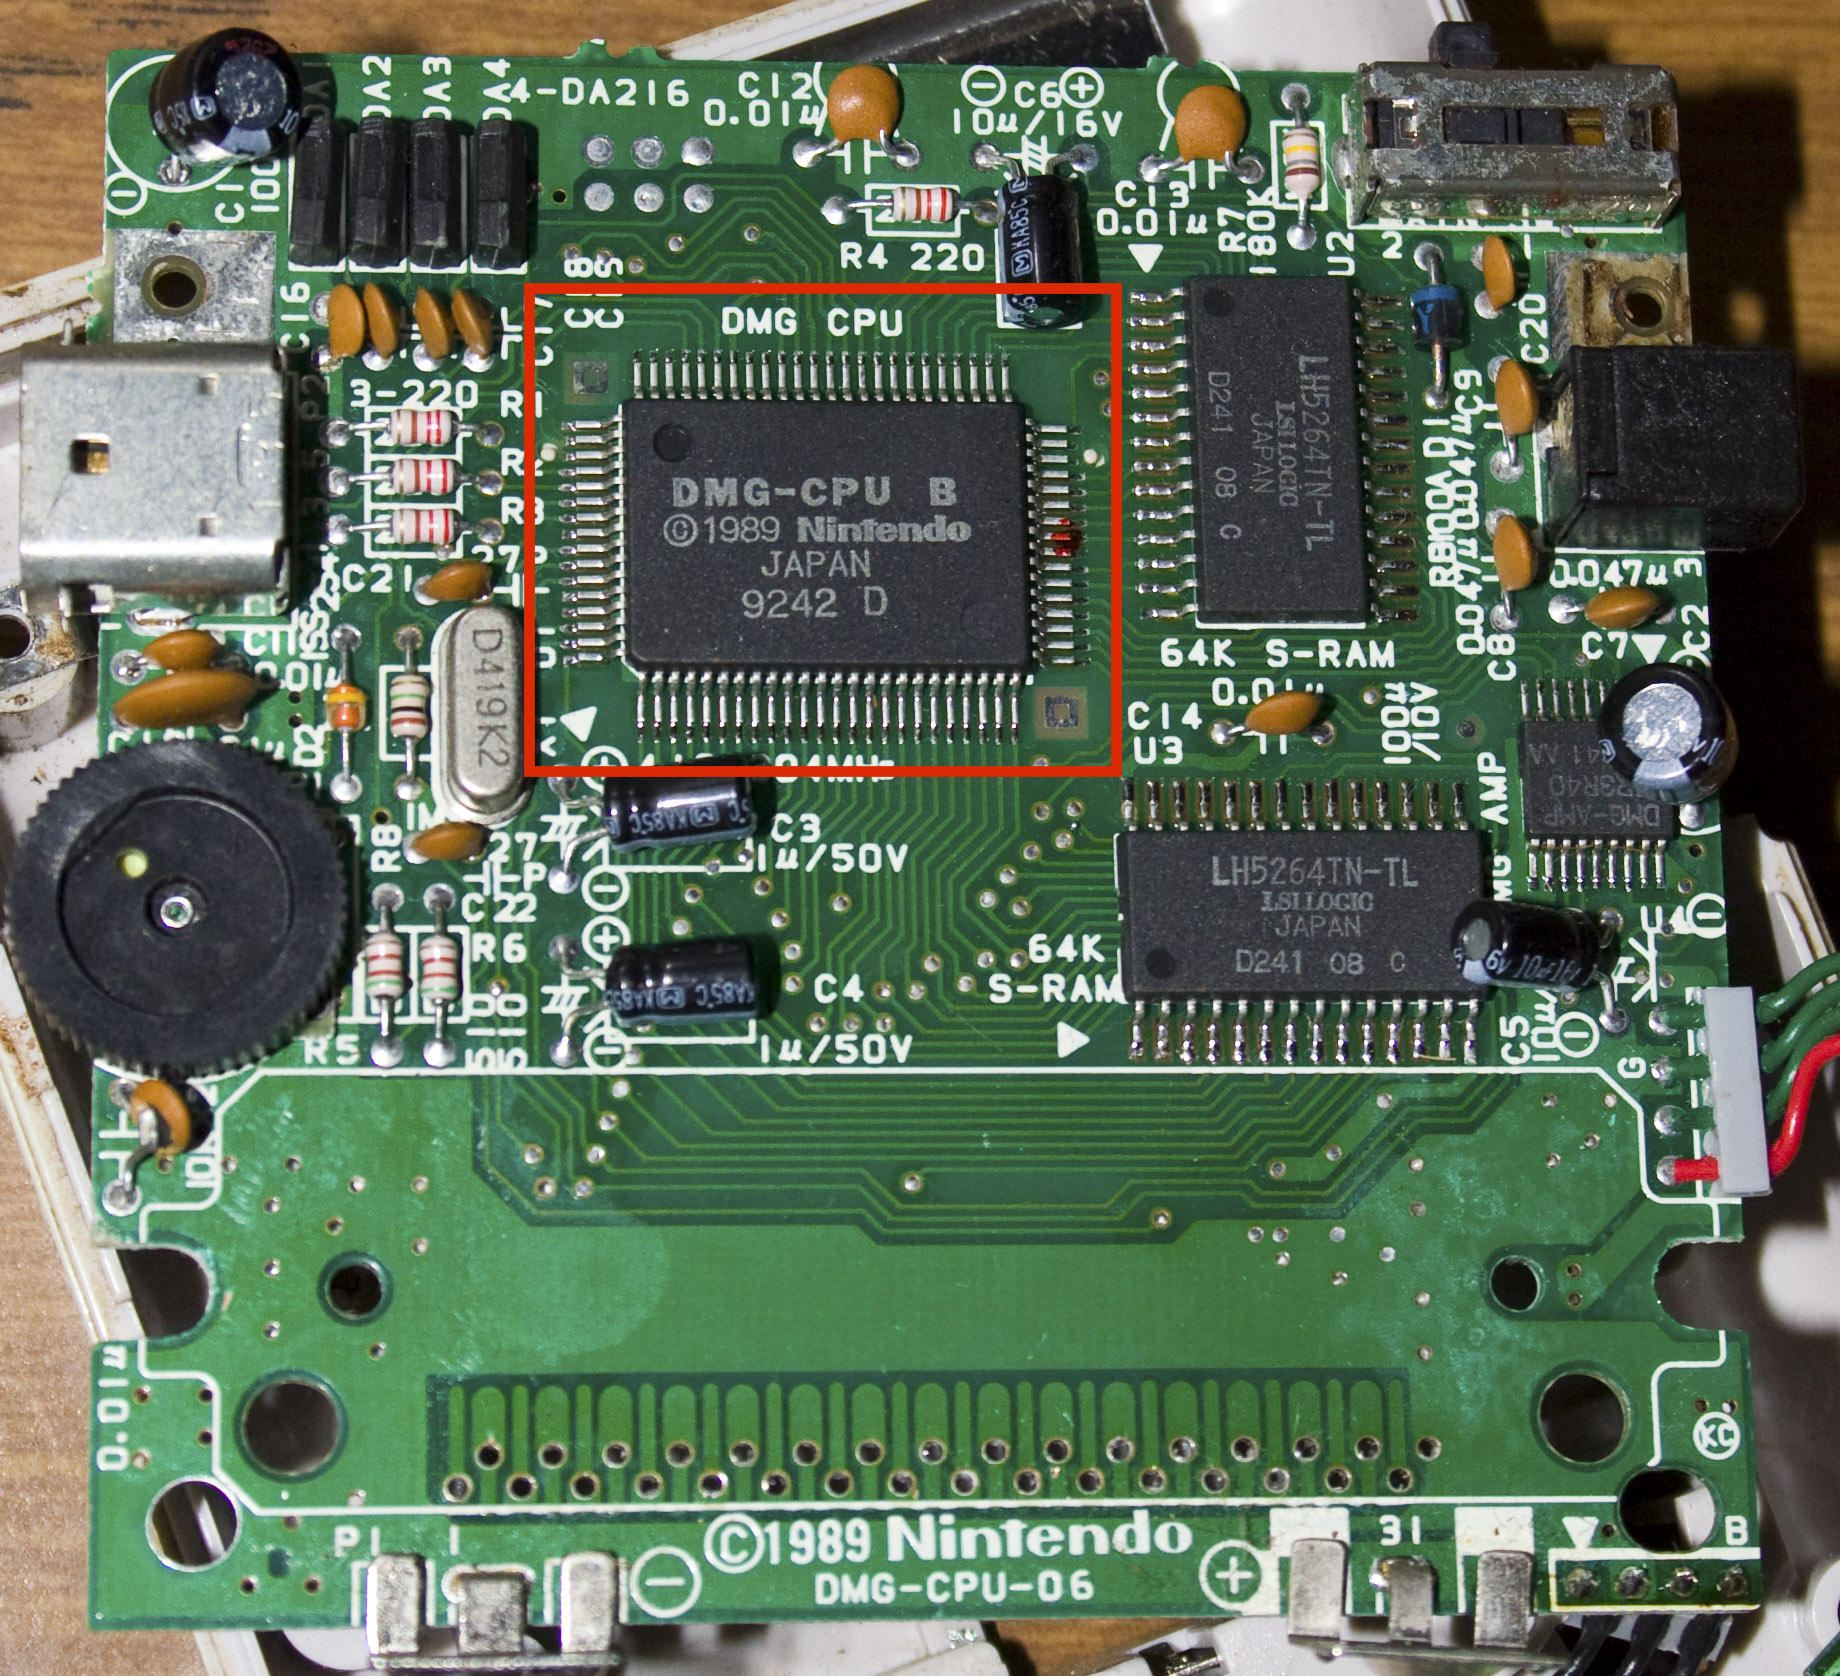
\includegraphics[scale=0.1]{images/cpu.jpg}
  \caption{Le processeur de la Gameboy}
\end{figure}

\subsubsection{Architecture}
Comme dit précédemment, le processeur de la Gameboy est semblable au Zilog Z80.
C'est en fait un hybride entre le Zilog Z80 et le Intel 8080. Le Intel 8080 a été
conçu pour être compatible avec le Zilog Z80 ce qui veut dire que les instructions
du 8080 sont aussi présentes dans le Z80. Le nom de ce processeur hybride est Sharp
LR35902. \\

Le processeur de la Gameboy est un processeur 8 bits avec 16 bits de bus d'adresse.
Il utilise 6 registres de 16 bits dont 4 pouvant être séparés en deux registres de
8 bits. Il donne aussi accès à 256 instructions ($2^{8}$) plus 256 instructions
supplémentaires et ses 16 bits de bus d'adresse permet d'adresser 64kB de mémoire.
Regardons maintenant plus en détail les regsitres du LR35902.

\subsubsection{Registres}
Ci-dessous, un tableau explicatif des 6 registres du processeur de la Gameboy.
\begin{center}
	\scalebox{1}{
		\begin{tabular}{| C{4cm} | C{4cm} | C{4cm} |}
			\hline
			Registres & 15:8 & 7:0 \\ \hline
			AF & A : registre & F : flags \\ \hline
			BC & B : registre & C : registre \\ \hline
			DE & D : registre & E : registre \\ \hline
			HL & H : registre & L : registre \\ \hline
			SP & \multicolumn{2}{c|}{Stack pointer} \\ \hline
			PC & \multicolumn{2}{c|}{Program counter} \\ \hline
		\end{tabular}
	}
\end{center}
Les regsitres, A, BC, DE et HL sont les registres de travail donc utilisés pour
toutes les opérations du programme. Le registre F contient les flags du processeur.
Il y a 4 flags différents.
\begin{itemize}[label=\textbullet]
	\item Z (Zero flag), qui indique si le résultat de la dernière opération était 0
	\item N (Negative flag), qui indique si le résultat de la dernière opération était négatif
	\item H (Halfcarry flag), qui indique s'il y a eu une retenue sur les 4 premiers bits
	\item C (Carry flag), qui indique s'il y a eu une retenue
\end{itemize}
Note: le Halfcarry flag était en général utilisé pour les affichages en décimal sur
l'écran (par exemple le score du joueur).

\subsubsection{Instructions}
Nous avons vu plus haut que le processeur de la Gameboy donnait accès à $256 \times 2$
instructions alors qu'une instruction était sur 8 bits. L'instruction 0xCB était
en fait une instruction préfix. Toute instruction donnée après ce prefix faisait
partie des 256 instructions supplémentaires. Nous verrons un exemple d'instruction
plus bas. Regardons d'abord le jeu d'instructions de la Gameboy et divisons les en catégories.
\paragraph{Instructions arithmériques}
\begin{itemize}[label=\textbullet]
	\item INC, incrémentation du registre
	\item DEC, décrémentation du registre
	\item ADD, addition de deux registres
	\item SUB, soustraction de deux registres
	\item ADC, addition de deux registres et du carry flag
	\item SBC, soustraction de deux registres et du carry flag
\end{itemize}
\paragraph{Opérations logiques}
\begin{itemize}[label=\textbullet]
	\item AND, ET bit à bit
	\item OR, OU bit à bit
	\item XOR, OU exclusif bit à bit
\end{itemize}
\paragraph{Opérations sur les bits}
\begin{itemize}[label=\textbullet]
	\item RL, rotation à gauche
	\item RR, rotation à droite
	\item SL, décalage à gauche
	\item SR, décalage à droite
	\item SWAP, inversion des bits
	\item BIT, teste un bit
	\item SET, set un bit
	\item RES, reset un bit
\end{itemize}
\paragraph{Sauts}
\begin{itemize}[label=\textbullet]
	\item JP, saut absolu à une adresse
	\item JR, saut relatif
	\item CALL, saut et stockage du program counter sur la pile (appel de fonction)
	\item RET, saut à l'adresse stockée dans la pile (retour de fonction)
\end{itemize}
\paragraph{Opérations avec la pile}
\begin{itemize}[label=\textbullet]
	\item PUSH, stockage d'un registre dans la pile
	\item POP, récupération de la dernière donnée empilée
\end{itemize}
\paragraph{Commandes processeur}
\begin{itemize}[label=\textbullet]
	\item NOP, pas d'opération
	\item HALT, arrête le processeur jusqu'à la prochaine interruption
	\item STOP, arrête le processeur
	\item EI, active une interruption
	\item DI, désactive une interruption
\end{itemize}
\paragraph{Autres instructions}
\begin{itemize}[label=\textbullet]
	\item LOAD, stockage d'une donnée depuis ou dans la mémoire
	\item CP, comparaison de deux registres
	\item DAA, conversion du registre A en décimal
\end{itemize}

\paragraph{Exemples d'instructions}
\begin{itemize}[label=\textbullet]
	\item 0x11 0x10 0x10 $\rightarrow$ LD DE, 0x1010
	\item 0xCB 0xC0 $\rightarrow$ SET 0, B
\end{itemize}

\newpage

%%%%%%%%%%%%%%%%%%%%%%%%%%%%%%%%%%%%%%%%%%%%%%%%%%%%%%%%%%%%%%%%%%

\subsection{Mémoire}

\begin{figure}[!h]
  \centering
  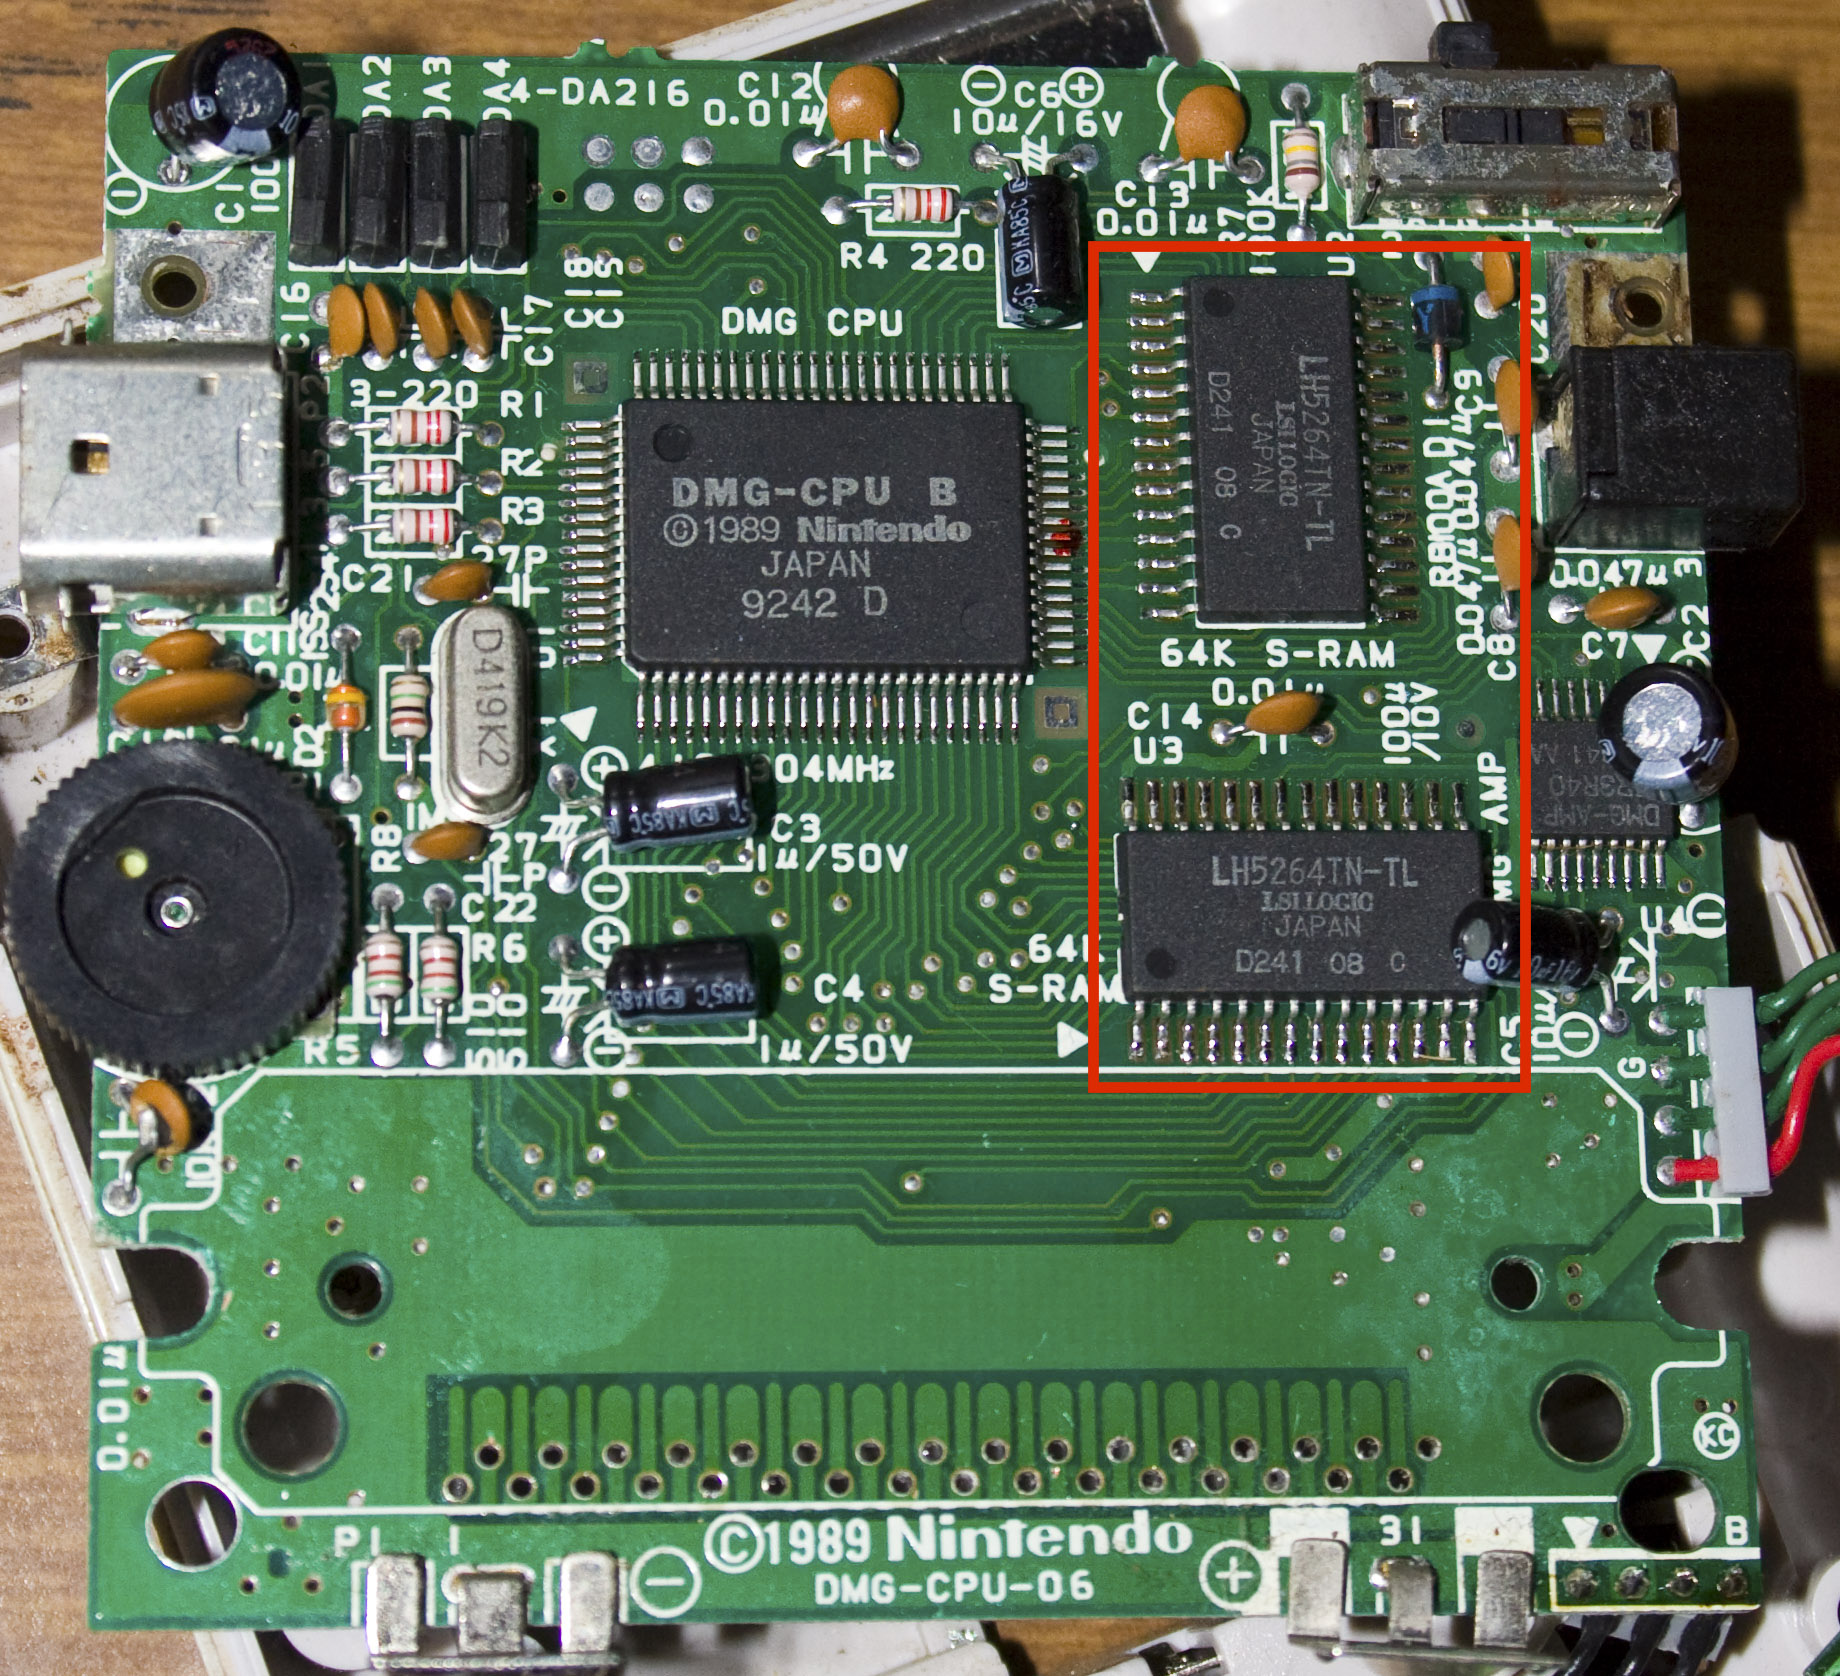
\includegraphics[scale=0.1]{images/mem.jpg}
  \caption{La mémoire de la Gameboy}
\end{figure}

\subsubsection{Memory map}
Nous avons vu à plusieurs reprises que la Gameboy avait une mémoire de 64kB.
Voyons plus en détail la structure de cette mémoire.
\begin{center}
	\scalebox{1}{
		\begin{tabular}{| C{4cm} | C{4cm} | c |}
			\hline
			Adresses & Nom & Description \\ \hline
			0000h – 3FFFh & ROM0 & ROM non-échangeable \\ \hline
			4000h – 7FFFh & ROMX & ROM échangeable \\ \hline
			8000h – 9FFFh & VRAM & Video RAM \\ \hline
			A000h – BFFFh & SRAM & RAM externe \\ \hline
			C000h – CFFFh & WRAM0 & Work RAM \\ \hline
			D000h – DFFFh & WRAMX & Work RAM échangeable \\ \hline
			E000h – FDFFh & ECHO & Echo de la WRAM \\ \hline
			FE00h – FE9Fh & OAM & Sprites \\ \hline
			FEA0h – FEFFh & UNUSED & - \\ \hline
			FF00h – FF7Fh & I/O Registers & - \\ \hline
			FF80h – FFFEh & HRAM & RAM interne du CPU \\ \hline
			FFFFh & IE Register & Registre d'activation des interruptions \\ \hline
		\end{tabular}
	}
\end{center}

\subsubsection{Cartouche}

La cartouche est un périphérique externe sur la Gameboy originale. Tout le code
qui est executé par la Gameboy est contenu dans la cartouche. Le jeu est mappé 
dans les 32 premiers kB de la mémoire de la console. Le problème qui se pose ici
est que les jeux ne peuvent faire une taille que de 32kB si on ne prend en compte
que cette information. Pour résoudre ce problème, la Gameboy met à disposition 
un mécanisme d'échanges de blocs mémoires entre sa mémoire et la mémoire du jeu 
(appelé MBC). \\

Ces échanges se font aux adresses allant de 0x4000 à 0x7FFF. Il existe de nombreux 
types de MBC dont la liste est disponible sur internet. Afin de savoir à quel type 
de MBC nous avons à faire, il faut lire à l'adresse 0x147. Il faut écrire à une 
adresse entre 0x2000 et 0x4000 pour changer de banque de ROM et écrire entre 0x4000 
et 0x6000 pour changer de banque de RAM. L'échange de banques de RAM n'est pas activé 
par défaut. Le jeu doit d'abord écrire 0xA à une adresse entre 0x0000 et 0x2000. 
A noté que toutes ces écritues ne sont pas effectives, elle permettent juste de 
gérer les banques de mémoire. Aucune donnée n'est écrite en ROM.

\newpage

\subsubsection{Bootstrap}
Dans la partie précédente, nous avons vu que les 32 premiers kB du jeu étaient mappés
au début de la mémoire de la console. Le seul moment ou ce n'est pas le cas est 
durant le démarrage de la console. Lors du démarrage de la console, le processeur
exécute un petit bout de code allant de 0x0 à 0x100. Ce bout de code est stocké en
dur dans la console et permet d'initialiser les registres et la mémoire de la Gameboy.
Le code de bootstrap n'a jamais été donné par Nintendo et n'a été que récemment
décodé par la communauté de développeurs. Ce code est donc mappé dans les 256 premiers
bytes de la console, le program counter commence à 0 puis après avoir executé l'ensemble
des instructions, il arrive à 0x100. L'éxécution du bootstrap était représenté par
un scroll du logo de Nintendo sur l'écran. Ensuite, Le bootstrap est retiré et le jeu peu
commencer son éxécution. A noter que le code du jeu commence donc à l'adresse
0x100. Les 256 premiers bytes contiennent les routines d'interruption.
\newline
\begin{figure}[!h]
  \centering
  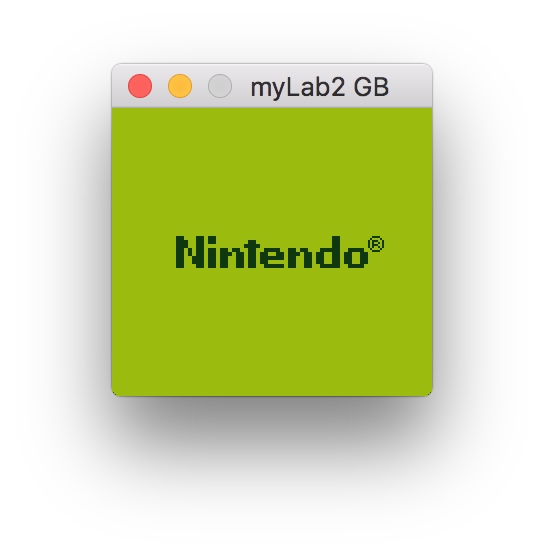
\includegraphics[scale=0.6]{images/bootstrap.png}
  \caption{Logo de Nintendo lors de l'exécution du bootstrap}
\end{figure}

\subsubsection{DMA}
Le registre DMA (0xFF46) permet d'activer le transfert DMA, entre tout adresse
(entre 0x0 et 0xF19F) et l'OAM (mémoire contenant les sprites). Le transfert commence
quand l'adresse source st écrite dans le registre DMA. Etant donné que le registre
ne fait que 8 bits, l'adresse source est multipliée par 0x100 et donne la réelle
adresse de départ du transfert. \\

Une fois que le transfert DMA commence, les données commençant à l'adresse
écrite dans le registre DMA sont écrites dans la région OAM de la mémoire.
Il y a 160 bytes écrits lors de ce transfert (taille de la région OAM).  L'avantage 
du DMA est de permettre de copier l'intégralité des données de sprites en une seule 
instruction au lieu d'avoir à faire 160 instructions à la suite.

%%%%%%%%%%%%%%%%%%%%%%%%%%%%%%%%%%%%%%%%%%%%%%%%%%%%%%%%%%%%%%%%%%

\subsection{Interruptions}

\subsubsection{Activer une interruption}
La Gameboy est capable de générer 5 types d'interruptions pour certains de ses
périphériques. Ces interruptions peuvent être contrôlées depuis deux registres
contenus dans la mémoire. Le registre IE (0xFFFF) et le registre IF (0xFF0F).
Les 5 premiers bits de ces deux registres représentent chacun une interruption.
\begin{center}
	\scalebox{1}{
		\begin{tabular}{| C{4cm} | C{4cm} | C{4cm} |}
			\hline
			Bit & Interruption & Adresse \\ \hline
			0 & V-Blank & 40h \\ \hline
			1 & LCD & 48h \\ \hline
			2 & Timer & 50h \\ \hline
			3 & Serial & 58h \\ \hline
			4 & Joypad & 60h \\ \hline
		\end{tabular}
	}
\end{center}
Ici, l'adresse est l'adresse dans la mémoire qui contient la routine d'interruption
(comme expliqué en 3.3.2). Le registre IE (Interrupt Enable) est modifié par le jeu.
Le registre IF (Interrupt Flag) quand à lui est modifié par les périphériques lorsqu'une 
interruption est demandée. \\

La dernière chose à savoir sur la gestion des interruptions est le "interrupt master".
Il n'est pas contenu dans la mémoire de la console et est un simple booléen que les
jeux mettent à 1 ou à 0. Si il est à 1, aucune interruption ne pourra être traité.
C'est donc un interrupteur qui est mis à 0 ou à 1 par les instructions EI, DI ou RETI.

\subsubsection{Demander une interruption}
Comme dit précédemment, un périphérique demande une interruption en modifiant le
bon bit dans le registre IF. Lorsqu'une interruption est demandée, elle n'est pas
forcemment traitée directement par le CPU. Tant que l'interruption n'est pas traitée,
le flag d'interruption doit resté à 1. De plus, lorsque un bit du registe IF est mis
à 1 par un périphérique que le même bit dans le registre IE est aussi à 1 et que
le CPU exécute l'instruction EI, le CPU ne sautera pas à la routine d'interruption
directement mais au prochain cycle d'horloge. A noter que cette particularité vaut 
pour l'instruction EI mais pas pour l'instruction RETI. Cette dernière retourne à
la dernière adresse mise dans la pile mais active les interruptions au coup d'horloge
actuel. \\

Exemple avec EI: \newline
\mintinline{c}{di} \newline
\mintinline{c}{ld a, 4h} \newline
\mintinline{c}{ld [FFFFh], a} \newline
\mintinline{c}{ld [FF0Fh], a} \newline
\mintinline{c}{ei} \newline
\mintinline{c}{inc a // cette instruction va être exécutée avant la routine d'interruption} \newline
\mintinline{c}{inc a // cette instruction va être exécutée après la routine d'interruption} \newline

Exemple avec RETI: \newline
\mintinline{c}{di} \newline
\mintinline{c}{ld a, 4h} \newline
\mintinline{c}{ld [FFFFh], a} \newline
\mintinline{c}{ld [FF0Fh], a} \newline
\mintinline{c}{reti} \newline
\mintinline{c}{inc a // cette instruction va être exécutée après la routine d'interruption} \newline
\mintinline{c}{inc a} \newline

\subsubsection{Traiter une interruption}
Nous avons pu voir qu'une interruption est traitée que si les bits correspondant
sont actifs dans les registres IE et IF mais aussi que le "interrupt master" (IME) est
à 1. La program counter est mis sur la pile puis il prend la valeur de l'adresse 
de la routine d'interruption demandée, IME est mis à 0 et le 
bit correspondant à l'interruption est mis à 0 dans le registre IF. Les routines
d'interruption terminent normalement par une instruction RET ou RETI. Dans le cas
de l'instruction RET, les interruption ne sont pas réactivées. Par contre, RETI
les réactive (IME à 1) ce qui permet à une autre interruption d'être
traitée (si par exemple un autre périphérique avait demandé une interruption en même
temps que le premier). Les priorités de traitement d'une interruption est dans l'ordre
du tableau ci-dessus. Le bit de poids faible a donc la plus grande priorité et ainsi
de suite.

\newpage

\subsubsection{Comportement de HALT}
L'instruction HALT est une instruction particulière car elle arrête le processeur
jusqu'à qu'une interruption a lieu. Son comportement varie en fonction de l'état
des registes IE, IF et du IME. L'instruction a en fait 3 comportements
différents.
\begin{itemize}[label=\textbullet]
	\item IME = 1
	\begin{itemize}[label=\textbullet]
		\item L'instruction HALT est exécutée normalement, le CPU s'arrête jusqu'à
		ce que deux bits correspondants soient mis à 1 dans IE et IF. Une fois fait,
		le CPU repart et saute directement à la routine d'interruption.
	\end{itemize}
	\item IME = 0
	\begin{itemize}[label=\textbullet]
		\item Si deux bits correspondants ne sont pas encore à 1 dans IE et IF, HALT 
		s'exécute normalement, comme lorsque IME = 1 sauf qu'une fois le CPU reveillé,
		l'exécution du programme continue (sans routine d'interruption).
		\item Si deux bits correspondants sont déjà à 1 dans IE et IF, le bug de HALT
		se produit. L'instruction HALT n'est pas exécutée et le processeur n'incrémente
		pas le program counter. L'instruction après l'instruction HALT est donc exécutée
		deux fois.
	\end{itemize}
\end{itemize}

%%%%%%%%%%%%%%%%%%%%%%%%%%%%%%%%%%%%%%%%%%%%%%%%%%%%%%%%%%%%%%%%%%

\subsection{Timer}
\subsubsection{Fonctionnement}
La Gameboy possède un timer qui compte à une certaine fréquence et provoque une
interruption lorsqu'il dépasse la limite du registre (overflow). Le timer se trouve
à l'adresse 0xFF05 de la mémoire (TIMA). Sa fréquence est donné par les deux premiers
bits du registre contrôle situé à l'adresse 0xFF07 (TAC). Le registre TIMA est sur 8 bits donc
sa valeur maximale est 255. Lorsque TIMA dépasse cette valeur la requête d'interruption
est envoyé et TIMA prend la valeur contenu par le registre à l'adress 0xFF06 (TMA).
On peut donc dire que TMA est le registre d'initialisation du timer. Il y a un
dernier registre lié au timer situé à l'adresse 0xFF04 appelé le divider register
(DIV). Nous verrons l'utilité de ce registre plus en détail après. Pour résumer :
\begin{center}
	\scalebox{1}{
		\begin{tabular}{| C{4cm} | C{4cm} | C{4cm} |}
			\hline
			Registre & Adresse & Description \\ \hline
			DIV & FF04h & Divider register \\ \hline
			TIMA & FF05h & Timer counter \\ \hline
			TMA & FF06h & Timer modulo \\ \hline
			TAC & FF07h & Timer controller \\ \hline
		\end{tabular}
	}
\end{center}

\subsubsection{Timer controller}
Le timer controller permet de fixer la fréquence du timer. Cette dernière peut être
de 4096Hz, 262144Hz, 65536Hz ou 16384Hz. C'est aussi dans ce registre qu'il est indiqué
si le timer est activé. C'est le bit 2 qui donne cette information (à 1 le timer
est activé et à 0 il ne l'est pas). Le deux bits de poids faible du registre TAC
indiquent à quelle fréquence va être incrémenté le timer.
\begin{center}
	\scalebox{1}{
		\begin{tabular}{| C{4cm} | C{4cm} |}
			\hline
			TAC[1:0] & Fréquence \\ \hline
			00 & 4096Hz \\ \hline
			01 & 262144Hz \\ \hline
			10 & 65536Hz \\ \hline
			11 & 16384Hz \\ \hline
		\end{tabular}
	}
\end{center}

\subsubsection{Divider register}
Le divider register est semblable au registre TIMA sauf que son incrémentation
ne dépend pas du registre TAC. Ce registre est incrémenté dans tous les cas à une 
fréquence de 16382Hz et est toujours actif, même si le timer est désactivé. Ce registre
était surtout utilisé pour la génération de nombres pseudo aléatoires. En effet, étant
donné qu'il est incrémenté constamment à partir du démarrage de la console, il
est très dur de prévoir quelle sera sa valeur. A noter que ce registre est remis
à 0 si le jeu tente d'écrire dedans (à partir d'une instruction LOAD par exemple).

%%%%%%%%%%%%%%%%%%%%%%%%%%%%%%%%%%%%%%%%%%%%%%%%%%%%%%%%%%%%%%%%%%

\subsection{GPU}
\subsubsection{Contrôleur LCD}
L'écran LCD de la Gameboy a une résolution de $160 \times 144$. L'écran LCD peut
être activé ou désactivé en modifiant le bit 7 du registre à l'adresse 0xFF40 appelé
LCD control (LCDC). L'écran est activé lorsque ce bit est à 1. Si le LCD est activé,
le controlleur de l'écran scanne ligne par ligne donc il y a théoriquement 144 lignes
à scanner. Cependant, le compteur de ligne (LY) situé à l'adresse 0xFF44 de la mémoire
va de 0 à 153. Les 8 lignes entre 144 et 153 sont des lignes qui n'existent pas mais
qui premettent au controlleur LCD d'entrer dans ce qui est appelé la V-Blank period.
Cette uné période où la mémoire vidéo de la console (VRAM) et la mémoire de sprites 
(OAM) peuvent être modifiés par le CPU. Lorsque le LCD arrive dans la V-Blank period,
une requête d'interruption est envoyé. De plus, comme pour le registre DIV du timer,
le registre LY est remis à 0 si le jeu essaye d'écrire dedans (par une instruction 
LOAD par exemple). \\

Nous avon vu un état du controlleur de l'écran LCD qui est le V-Blank mais il a 
en fait 4 états différents.  H-Blank, V-Blank, recherche de sprites et transfert
des données au LCD. Ces états sont indiqués dans le registre à l'adresse 0xFF41
(STAT). Les deux bits de poids faible de ce registre représentent l'état actuel
du controlleur.
\begin{center}
	\scalebox{1}{
		\begin{tabular}{| c | c | C{9cm} |}
			\hline
			STAT[1:0] & État & Description \\ \hline
			00 & H-Blank & La VRAM et l'OAM peuvent être modifiées par le CPU \\ \hline
			01 & V-Blank & La VRAM et l'OAM peuvent être modifiées par le CPU et l'écran est désactivé\\ \hline
			10 & Recherche de sprites & Le controlleur lit l'OAM qui est donc inaccessible par le CPU \\ \hline
			11 & Transfert des données & Le controlleur lit l'OAM et la VRAM qui sont donc inaccessibles par le CPU \\ \hline
		\end{tabular}
	}
\end{center} \bigbreak

Lorsqu'une nouvelle ligne est scannée, le controlleur entre dans l'état 2 puis il
passe au 3 et enfin au 0. Ce pattern est ensuite répété jusqu'à ce que le controlleur
arrive en V-Blank period et passe à l'état 1. Tout est recommencé une fois le V-Blank
passé. Il faut 456 coups d'horloge pour scanner une ligne et passer à la suivante.
Ce qui sépare le nombre de cycles passés à chaque état de cette manière:
\begin{itemize}[label=\textbullet]
	\item 80 coups d'horloge pour l'état 2
	\item 172 coups d'horloge pour l'état 3
	\item 204 coups d'horloge pour l'état 0
\end{itemize} \bigbreak

Lors d'un changement d'état (par exemple lors du passage du mode 1 au mode 2),
le controlleur LCD peut demander une interruption. Les bits 3, 4 et 5 du registre
STAT permettent d'activer ces interruptions. Le bit 3 autorise l'interruption lors
du passage au mode 0, le bit 4 lors du passage au mode 1 et le bit 5 lors du passage
au mode 2. Il n'y a pas d'interruption possible lors du passage au mode 3. \\

Un dernier registre est lié au controlleur LCD, le registre à l'adresse 0xFF45
appelé LY compare (LYC). Si les registres LY et LYC on la même valeur, le bit 2
du registre STAT est mis à 1. Si ce bit est à 1 est que son bit d'interruption associé,
le bit 6, est aussi à 1 alors une interruption est demandé. Cette interruption
permet au jeu de savoir quand une ligne est scannée pour faire certains effets.

\subsubsection{Affichage}
\paragraph{Contrôle de l'affichage} \mbox{} \\

Nous avons vu précedemment que l'écran LCD de la Gameboy a pous résolution
$160 \times 144$. Ceci est partiellemnt vrai. Physiquement, l'écran a ces dimensions
mais dans la mémoire, l'écran a une résolution de $256 \times 256$. Ces pixels
supplémentaires permettent le scrolling des éléments de fond de l'affichage. Le
scrolling se fait à l'aide de deux registres, SCROLLY et SCROLLX situés respectivement
aux adresses 0xFF42 et 0xFF43. Ces $256 \times 256$ pixels sont rassemblés en $32 \times 32$ tiles.
Une tile fait donc $8 \times 8$ pixels. En plus de cette zone de fond, l'affichage de la
Gameboy possède aussi une zone appelé window (ou fenêtre). La fenêtre est composée
de tiles, comme le fond sauf que cet élément est fixe, il ne peut pas être scrollé.
La position de la fenêtre sur l'écran est définie à l'aide des registres WINDOWY
et WINDOWX situés respectivement aux adresses 0xFF4A et 0xFF4B.
L'interêt d'une zone fixe est l'affichage d'éléments fixes comme le score du joueur,
sa vie, etc... Le dernier élément graphique qui a déjà été vu plus haut est le sprite.
Un sprite représente tous les objets en mouvement sur l'écran (personnage contrôllé par
le joueur, ennemis, briques de Tetris, etc...). \\

Pour résumer nous avons les éléments suivants:
\begin{itemize}[label=\textbullet]
	\item Backgroud : La zone de fond scrollable
	\item Window : La fenêtre fixe par dessus le fond
	\item Sprites : Les objets en mouvement
\end{itemize} \bigbreak

Afin de savoir où se trouvent tous ces éléments graphique dans la mémoire, il faut
regarder dans le registre LCDC (0xFF40). Ci-dessous l'explication sur l'utilité
de chacun de ses bits.
\begin{center}
	\scalebox{1}{
		\begin{tabular}{| c | c | c | c |}
			\hline
			Bit & Nom & \multicolumn{2}{c|}{États} \\ \hline
			7 & LCD Enable & 0 : Off & 1 : On \\ \hline
			6 & Window Tile Map Display Select & 0 : 9800h-9BFFh & 1 : 9C00h-9FFFh \\ \hline
			5 & Window Display & 0 : Off & 1 : On \\ \hline
			4 & BG / Window Tile Data Select & 0 : 8800h-97FFh & 1 : 8000h-8FFFh \\ \hline
			3 & BG Tile Map Display Select & 0 : 980h0-9BFFh & 1 : 9C00h-9FFFh \\ \hline
			2 & OBJ (Sprite) Size & 0 : 8x8 & 1 : 8x16 \\ \hline
			1 & OBJ (Sprite) Display Enable & 0 : Off & 1 : On \\ \hline
			0 & BG / WindowDisplay & 0 : Off & 1 : On \\ \hline
		\end{tabular}
	}
\end{center}

\paragraph{Afficher le background et la fenêtre} \mbox{} \\

On peut déjà remarquer que les bits 6, 4 et 3 indiquent des adresses en mémoire.
Ce sont les adresses où seront situées les données indispensables à l'affichage.
Les tile map sont des ensemble d'identifiant de tiles. L'identifiant permet de
trouver la tile à afficher dans la data table qui contient les données des pixels
de tous les tiles possible du jeu. L'identifiant est sur 8 bits mais est signé si
les données sont situées entre  0x8800 et 0x97FF. Dans le cas contraire, l'identifiant
est non signé. \\

Une fois l'identifiant trouvé, il faut afficher les données contenues
dans la data table. Un pixel de l'écran de la Gameboy est codé sur deux bits et
une tile est composé de $8 \times 8$ pixels. Une ligne d'une tile fait donc 16 bits.
Il faut combiner ces 16 bits pour avoir la bonne information sur les pixels de la ligne.
\begin{center}
	\scalebox{1}{
		\begin{tabular}{|c|c|c|c|c|c|c|c|c|}
			\hline
			Pixel & 1 & 2 & 3 & 4 & 5 & 6 & 7 & 8 \\ \hline
			Octet 1 & 1 & 0 & 1 & 0 & 1 & 1 & 1 & 0 \\ \hline
			Octet 2 & 0 & 0 & 1 & 1 & 0 & 1 & 0 & 1 \\ \hline
			Identifiant couleur & 2 & 0 & 3 & 1 & 2 & 3 & 2 & 1 \\ \hline
		\end{tabular}
	}
\end{center}
Finalement, pour avoir la valeur réelle du pixel il faut aller chercher dans la
palette de couleur située dans le registre à l'adresse 0xFF47 pour le background
et la fenêtre (les sprites peuvent avoir deux palettes de couleur différentes
mais nous verrons ça plus tard). Cette palette est sur 8 bits et l'identifiant
trouvé précedemment indique quelle paire de bits contient la couleur. 0 pour les
bits 0 et 1, 1 pour les bits 2 et 3, 2 pour les bits 4 et 5, 3 pour les bits 6 et 7.
La couleur ainsi récupérée est aussi sur deux bits.
\begin{itemize}[label=\textbullet]
	\item 00 : Blanc
	\item 01 : Gris clair
	\item 10 : Gris foncé
	\item 11 : Noir
\end{itemize} \bigbreak

\newpage

\paragraph{Afficher les sprites} \mbox{} \\

Les tiles des sprites sont toujours situées aux mêmes adresses entre 0x8000 et
0x8FFF. Il est donc plus simple de les trouver en comparaison du background
ou de la fenêtre. Il y a 40 tiles reservées au sprites et chaque sprite
est lié à une table d'attributs, 4 registres sur 8 bits situés entre les adresses
0xFE00 et 0xFE9F. Ces attributs sont, dans l'ordre, sa position en y, sa position
en x, son identifiant dans la data table et enfin un registre d'attributs. Les
4 bits de poids fort de ce registre d'attribtus sont utilisés par la Gameboy
et représentent, dans l'ordre, la priorité du sprite par rapport au background,
sa rotation en y, sa rotation en x et son numéro de palette de couleurs (nous avions
vu précedemment que les sprites avaient deux palettes de couleurs). Ces deux
palettes sont situées aux adresses 0xFF48 et 0xFF49. \\

Pour afficher les sprites du jeu il faut donc parcourir l'ensemble des sprites 
entre 0xFE00 et 0xFE9F et les afficher en utilisant leurs attributs. Le fonctionnement
de la palette de couleur est le même que pour le background et la fenêtre.

%%%%%%%%%%%%%%%%%%%%%%%%%%%%%%%%%%%%%%%%%%%%%%%%%%%%%%%%%%%%%%%%%%

\subsection{Entrées}
La gameboy possède 8 entrées différentes. La croix directionnelle et les boutons
A, B, START et SELECT. Leur contrôle se fait par l'intermédiaire d'un seul
registre en mémoire, le registre P1, situé à l'adresse 0xFF00. Ce registre
est structuré de cette manière :
\begin{center}
	\scalebox{1}{
		\begin{tabular}{| c | c | c | c |}
			\hline
			Bit & Nom & \multicolumn{2}{c|}{États} \\ \hline
			7 & Not used & \multicolumn{2}{c|}{-} \\ \hline
			6 & Not Used & \multicolumn{2}{c|}{-} \\ \hline
			5 & Select Button Keys & 0 : On & 1 : Off \\ \hline
			4 & Select Direction Keys & 0 : On & 1 : Off \\ \hline
			3 & Input Down or Start & 0 : Pressed & 1 : Not Pressed \\ \hline
			2 & Input Up or Select & 0 : Pressed & 1 : Not Pressed \\ \hline
			1 & Input Left or Button B & 0 : Pressed & 1 : Not Pressed \\ \hline
			0 & Input Right or Button A & 0 : Pressed & 1 : Not Pressed \\ \hline
		\end{tabular}
	}
\end{center}
On peut voir que la croix directionnelle et les boutons partagent les même bits
(de 3 à 0). C'est en fait le jeu qui va séléctionner quelles entrées vont l'intéresser
en séléctionnant les boutons ou la croix directionnelle avec les bits 5 et 4.
De plus, lors du passage d'une des entrées de l'état haut à l'état bas (donc lors
de la pression d'un bouton étant donné qu'ils sont actifs à l'état bas), une
interruption est demandé au processeur.

\newpage

%%%%%%%%%%%%%%%%%%%%%%%%%%%%%%%%%%%%%%%%%%%%%%%%%%%%%%%%%%%%%%%%%%
%%%%%%%%%%%%%%%%%%%%%%%%%%%%%%%%%%%%%%%%%%%%%%%%%%%%%%%%%%%%%%%%%%

\section{Émulateur}
\subsection{Introduction}
Une fois toutes ces informations trouvées sur la Gameboy il a fallut commencer
à développer l'émulateur. Ce dernier est divisé en 3 parties. La librairie de gestion
des périphériques de la MyLab2, la librairie d'émulation des périphériques de la Gameboy
et enfin le programme principal qui va utiliser ces deux librairies afin de faire
tourner l'émulateur sur la MyLab2. Chacun des périphériques de la MyLab2 et de la
Gameboy décrits  ci-dessus sont présents sous forme de modules dans ce deux librairies C.
Les algorithmes implémentés sont les même que ceux décrits dans les partie 2 et 3. \\

%%%%%%%%%%%%%%%%%%%%%%%%%%%%%%%%%%%%%%%%%%%%%%%%%%%%%%%%%%%%%%%%%%

\subsection{Librairie d'émulation de la Gameboy}

\begin{figure}[!h]
  \centering
  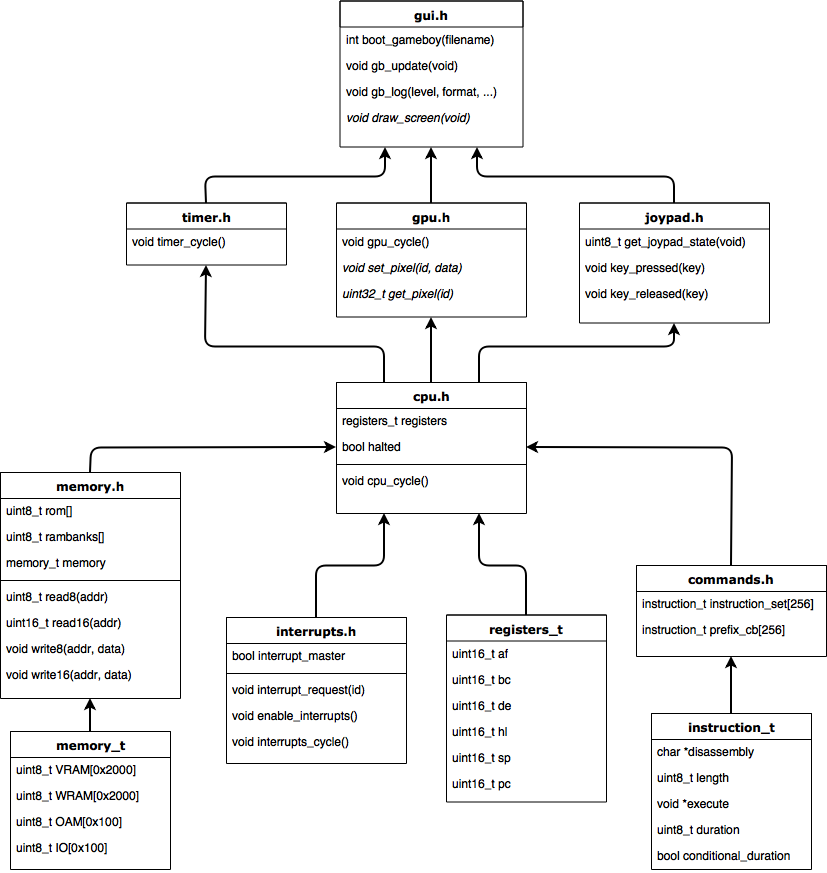
\includegraphics[scale=0.4]{images/class_diag.png}
  \caption{Diagramme de la librairie de la Gameboy}
\end{figure}

Le processeur est représenté sous forme de deux structures C. L'une représente
les registres et l'autre une instruction. Une instruction contient son nom, 
sa longueur, un pointeur vers une fonction, sa durée en cycles d'horloge de la Gameboy
et un booléen qui indique si la durée dépend du résultat de l'instruction (un saut
conditionnel par exemple ne prendre pas autant de cycles d'horloge si le saut se fait
ou non). Toutes les instructions sont stockées sous forme de tableau et permet
une grande flexibilité. Par exemple, si le program counter indique qu'il faut exécuter
l'instruction 0x11, il suffit de faire \mintinline{c}{instruction_set[0x11]}. Il
faut bien sûr prendre en compte la longueur de l'instruction ainsi que regarder
si l'instruction ne fait pas partie de l'extension d'instructions (prefixé par 0xCB)
mais dans l'idée c'est ce qu'il faut faire.

\newpage

La mémoire est accessible un peu moins facilement. En effet, à cause des problèmes 
de mémoire de la MyLab2, la ROM a été mise entièrement en constante afin qu'elle 
soit stockée dans la flash. De plus, toutes les zones mémoires non utilisées par 
la Gameboy n'ont pas été émulées. La structure C représentant la mémoire n'est 
donc pas continue (il ne suffit pas de faire mem[addr] pour accéder à la mémoire).
Ceci rend les accès mémoires un peu plus lent mais c'était indispensable pour faire
tourner l'émulateur sur le microcontrolleur. \\

Les modules du CPU, des interruptions, du timer et du GPU contiennent chacun une
fonction \mintinline{c}{cycle}. Ces 4 fonctions sont en fait appelées par la fonction
\mintinline{c}{gb_update} de \mintinline{c}{gui.h} dans une boucle infinie. Ces
fonctions permettent de mettre à jour l'état des périphériques qu'elles émulent.
La fonction \mintinline{c}{cpu_update} retourne le nombre de cycles d'horloges
théorique qu'aurait du prendre la Gameboy pour effectuer l'instruction actuelle.
A chaque cycle, ce nombre est ajouté à un total de nombres de cycles qui, une fois
arrivé à $\frac{4194304}{FREQ}$, affiche l'horloge et recommence à nouveau. Ici,
$FREQ$  est le nombre de raffraichissement de l'écran par seconde et $4194304$ est 
la fréquence réelle du processeur de la Gameboy (les 4,19MHz dont j'ai parlé plus haut).
Pour être plus précis, il faudrait calculer le temps réel passé à faire un \mintinline{c}{gb_update},
le soustraire à la période et endormir le programme le temps obtenu. Ce n'est pas
fait ici car l'émulateur est plus lent que la vraie Gameboy, il n'y a donc pas
besoin d'attendre. Ceci donne le schéma suivant. \\
\begin{figure}[!h]
  \centering
  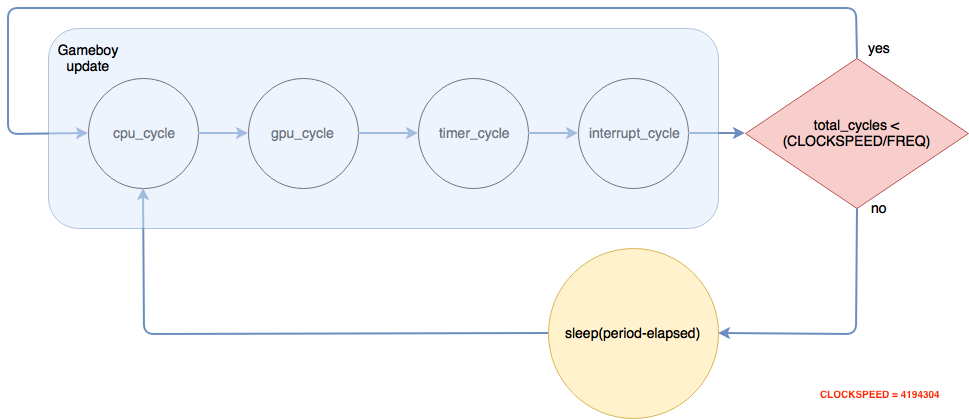
\includegraphics[scale=0.4]{images/schema.png}
  \caption{Schéma de déroulement de l'émulateur}
\end{figure}
\newline

Les fonctions écrites en italique dans le diagramme sont des fonctions non implémentées
dont seulement les prototypes sont données. Ceci n'a été fait que sur les fonctions
graphique \mintinline{c}{set_pixel}, \mintinline{c}{get_pixel} et \mintinline{c}{draw_screen}.
Ceci permet de réutiliser la librairie sur un autre environnement de programmation
en ne changeant que ces 3 fonctions. La librairie faite durant ce travail de semestre
peut ainsi être compilée dans un programme C sur un ordinateur. Il a juste fallut
faire des fonctions d'affichage en utilisant la librairie graphique SDL2 en plus.
Cette fonctionnalité m'a beaucoup aidé pour le debug étant donné la lenteur d'affichage
de la MyLab2. L'émulateur est donc multiplateforme. \\

Une dernière fonctionnalité de cette librairie est la possibilité de faire des logs.
La fonction \mintinline{c}{gb_log} affiche les différents états de l'émulateur
ainsi que les erreurs. Le niveau de log peut être choisi. Il y a 4 niveaux de log,
ERROR, WARNING, INFO, DEBUG et le niveau est à INFO par défaut. Lorsque l'émulateur
est compilé sur un ordinateur, les logs sont affichés sur stderr. Sur la MyLab2,
les logs sont envoyés sur l'UART avec un baudrate de 115200.

%%%%%%%%%%%%%%%%%%%%%%%%%%%%%%%%%%%%%%%%%%%%%%%%%%%%%%%%%%%%%%%%%%

\subsection{Programme principal}
Le programme principal est divisé en deux fichiers. \mintinline{c}{display.c}
et \mintinline{c}{controls.c}. Comme leurs noms l'indique, l'un gère les entrées
(joystick, boutons et dalle tactile) et l'autre l'affichage (écran LCD).
La MyLab2 a un joystick et les boutons A et B mais pas de boutons START et SELECT.
Ils sont émulés par deux boutons affichés sur l'écran tactile. \\

Le problème avec l'émulation des boutons sur l'écran tactile est que le bus I$^2$C
a besoin des interruptions pour fonctionner sauf que nous avons vu plus haut que 
la détection de l'écran marche avec une interruption GPIO. L'interruption I$^2$C 
ne se fera jamais tant que nous nous trouvons dans l'interruption $\overline{EINT3}$.
Il faut donc simplement avertir avec des flags si l'écran a été appuyé ou relaché
puis venir  vérifier ces flags régulièrement et appeler les fonctions de la dalle tactile.
Ici, ces flags sont vérifiés avec la même fréquence que le raffraichissement de
l'écran. Pour l'émulation graphique, il a fallut diminuer le plus possible le nombre 
d'écritures sur l'écran LCD. J'ai donc décidé de créer un tableau contenant les
données des $160 \times 144$ pixels de l'écran. Pour optimiser le plus possible 
l'espace, chaque pixel est sur deux bits dans ce tableau (comme pour la gameboy).
Voilà finalement à quoi ressemble le \mintinline{c}{main} du programme C flashé
sur la carte.

\inputminted[breaklines,breaksymbol=,linenos,frame=single,stepnumber=5,tabsize=2,firstline=14,lastline=35]
{c}{../../workspace/mylab2-gb/src/mylab2-gb.c}

%%%%%%%%%%%%%%%%%%%%%%%%%%%%%%%%%%%%%%%%%%%%%%%%%%%%%%%%%%%%%%%%%%

\subsection{Problèmes rencontrés}
\subsubsection{Limites de la MyLab2}
Durant tout le développement de l'émulateur, de nombreux problèmes ont été rencontrés.
Tout d'abord, j'ai vite été confronté aux limitations de la MyLab2. En effet,
son processeur n'est pas assez rapide pour émuler la Gameboy. Il faut 5sec à la
Gameboy pour passer le code de Bootstrap alors qu'il en faut 25 à la MyLab2 pour
faire la même chose. L'émulateur est donc 5 fois plus lent sur le microcontrolleur.
De plus, sa mémoire n'est pas suffisante pour accueillir l'intégralité de la mémoire
de la Gameboy. Comme déjà expliqué précedemment, j'ai du scinder la mémoire afin
de retirer les parties inutiles et mettre la ROM en flash. Même comme ça, les jeux
les plus lourds ne pourront jamais être émulés par la MyLab2 car il faudrait au moins
émuler 32kB de RAM pour la Gameboy. J'ai aussi essayé un moment d'utiliser le DMA
du LPC1769 afin de communiquer avec l'écran. Pour utiliser le DMA, il ne faut pas
utiliser l'interface SPI mais l'interface SSP0. Ce n'est qu'une fois l'implémentation
de la gestion du SSP0 que j'ai découvert un bug avec le SSP0 sur le LPC1769. La ligne
MOSI de l'interface reste toujours à l'état haut. Je n'ai donc pas pu utiliser le
DMA pour la communication avec l'écran LCD.

\subsubsection{Débogage de l'émulateur}
La Gameboy doit être une des consoles la plus émulée de part sa simplicité mais aussi
sa valeur nostalgique. Comme je l'ai déjà dit plus haut, ceci fait que l'on peut
trouver énomément de documentation sur internet voir même trop. Il a été difficile
de séparer les informations vraies des fausses. J'ai trouvé de nombreux documents,
projets ou blogs se contredisant les uns des autres. Il a donc fallut tester, voir
si le comportement est bien le bon mais même comme ça, il était difficile de vraiment
savoir si l'émulateur était juste (surtout avant l'implémentation de l'écran LCD).
Heureusement, des tests unitaires ont été développés par la communauté afin d'aider
dans le développement d'émulateurs. Ces tests sont les tests de Blargg et les tests
de Mooneye. J'ai personnellement plus travaillé avec les tests de Blargg car ils
sont plus globaux alors que ceux de Mooneye sont spécifique à des comportements précis
de la Gameboy. La première chose qu'il a fallut valider était l'implémentation
du CPU. Au départ les tests ne passaient pas mais c'est ainsi que j'ai pu trouver
des erreurs dans certaines implémentations d'instructions. Les tests de Blargg
affichent les résultats des tests sur l'écran mais pour ceux n'ayant pas encore
implémenté l'affichage, les résultats sont aussi écrites dans le registre SB, à
l'adresse 0xFF01 de la Gameboy. Si 0x81 est écrit dans le registre SC (adresse 0xFF02),
il faut venir lire le registre SB. Chaque donnée est un caractère du résultat
du test. Ces registres permettent normalement de contrôler la communication série
de la Gameboy.

%%%%%%%%%%%%%%%%%%%%%%%%%%%%%%%%%%%%%%%%%%%%%%%%%%%%%%%%%%%%%%%%%%

\subsection{Résultats}
\begin{figure}[!h]
  \centering
  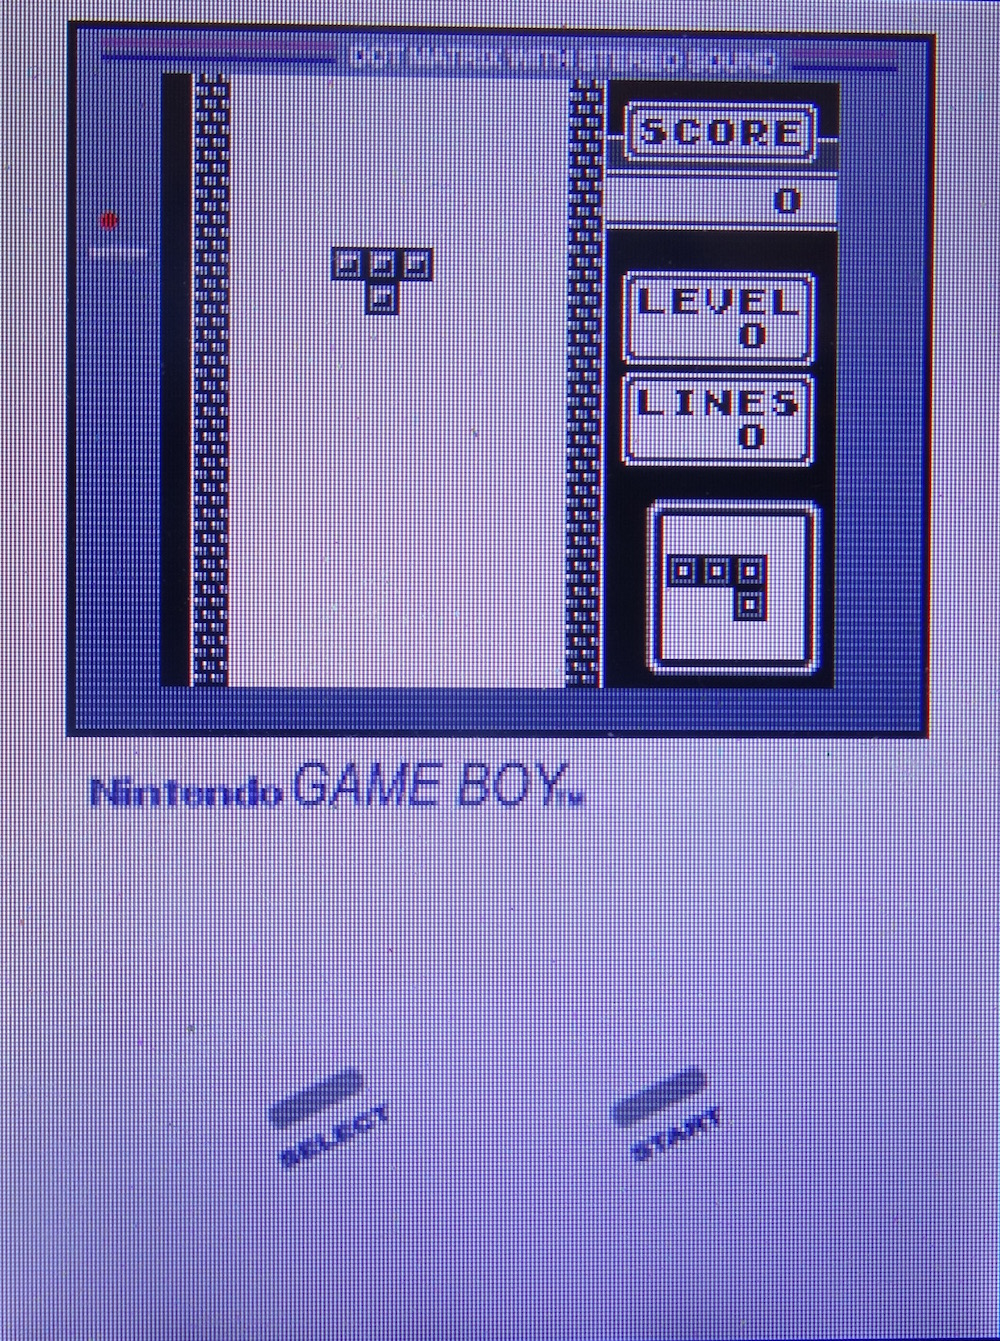
\includegraphics[scale=0.3]{images/mylab2gb.jpg}
  \caption{MyLab2 GB en marche}
\end{figure}
L'émulateur est entièrement fonctionnel sur la MyLab2. A noter que toutes les
composantes graphiques supplémentaires comme le logo de Nintendo ou l'indicateur
de batterie sont des fichiers bitmap mises en constantes dans le programme. Il
manque tout de même certaines choses comme le son ou la communcation série (on
pourrait imaginer deux MyLab2 pouvant communiquer). L'émulateur n'est donc pas fini
il permet de faire tourner certains jeux mais pas tous. L'émulation de toutes
les banques de mémoire est aussi à finir. Tout ce qui reste à faire est indiqué
sur la page Github du projet. Il faudrait aussi trouver une solution pour le
problème de latence.

\newpage

%%%%%%%%%%%%%%%%%%%%%%%%%%%%%%%%%%%%%%%%%%%%%%%%%%%%%%%%%%%%%%%%%%
%%%%%%%%%%%%%%%%%%%%%%%%%%%%%%%%%%%%%%%%%%%%%%%%%%%%%%%%%%%%%%%%%%

\section{Conclusion}
Bien que plus lent que la Gameboy originale, l'émulateur développé durant ce
semestre est finalement fonctionnel. Il peut encore y avoir un peu d'optimisation
mais au final il sera toujours plus lent. Une idée avait été de porter l'émulateur
sur la MyLab2 avec le LPC4337 qui est dual core. Même si les horloge des deux
processeurs de ce microcontrolleur ont une fréquence d'horloge plus élevée,
je pense que ça ne rendra toujours pas l'émulateur aussi rapide que l'original.
Nous avons vu plus haut que actuellement, l'émulateur est 5 fois plus lent que
normalement. Le LPC4337 et seulement 2 fois plus rapide que le LPC1769. Même
paralléliser les tâches ne servirait pas ici car ce n'est pas l'affichage qui
ralentit mais bien le travail d'émulation du CPU. L'émulateur serait juste
un peu plus jouable avec le LPC4337. \\

Une solution à laquelle j'ai pensé est de refaire entierement le processeur
de la Gameboy sur une FPGA. La FPGA serait connectée à la MyLab2 (par les pins
Pmod par exemple). La FPGA s'occuperait de toute la partie logique et la MyLab2
de tout l'affichage et des entrées. Une partie de l'émulateur fait durant ce 
semestre serait donc utilisable et toute la partie FPGA serait à faire. On pourrait
imaginer un nouveau travail de semestre portant sur ce sujet. \\

En conclusion, je dirais que ce projet a été très intéressant. Il m'a permis de
découvrir le fonctionnement d'une console à laquelle j'ai pu jouer par le passé.
J'ai aussi pu expérimenter les limites de la MyLab2 qui est une carte que nous
avons beaucoup utilisé en deuxième année. J'espère que des idées d'amélioration
pourront être trouvées afin d'avoir un émulateur réellement fonctionnel fait à hepia.

\newpage

%%%%%%%%%%%%%%%%%%%%%%%%%%%%%%%%%%%%%%%%%%%%%%%%%%%%%%%%%%%%%%%%%%
%%%%%%%%%%%%%%%%%%%%%%%%%%%%%%%%%%%%%%%%%%%%%%%%%%%%%%%%%%%%%%%%%%

\section{Références}
\nocite{*}
\bibliographystyle{unsrt}
\bibliography{biblio}

\end{document}
